\documentclass[UTF8]{ctexart}
\usepackage[table]{xcolor}
\usepackage{bm}
\usepackage{amssymb}
\usepackage{mathtools}
\usepackage{amsmath}
\usepackage{float}
\usepackage{rotating}
\usepackage{booktabs}
\usepackage{pdfpages}
\usepackage{subfigure}
\usepackage{mathtools}
\usepackage{amsmath}
\usepackage{listings}
\usepackage{fancybox}
%\usepackage{xcolor}
%\usepackage{colortbl}
\usepackage{diagbox}
\usepackage{amssymb}
\usepackage{warpcol}
\usepackage{lscape}
\usepackage[framemethod=tikz]{mdframed}
\usepackage{longtable,booktabs}

\title{\heiti 最优化第十五次作业}
\author{\kaishu 张晋15091060}
\begin{document}
\maketitle


\begin{enumerate}
\item[7.20]
函数$f(x)=\dfrac{1}{2}(\dfrac{1}{2}x^2-14)^2-x^2+3x$及其导数$f'(x)=\dfrac{1}{2}x^3-16x+3$的图像如下:


\begin{figure}[H]
\centering
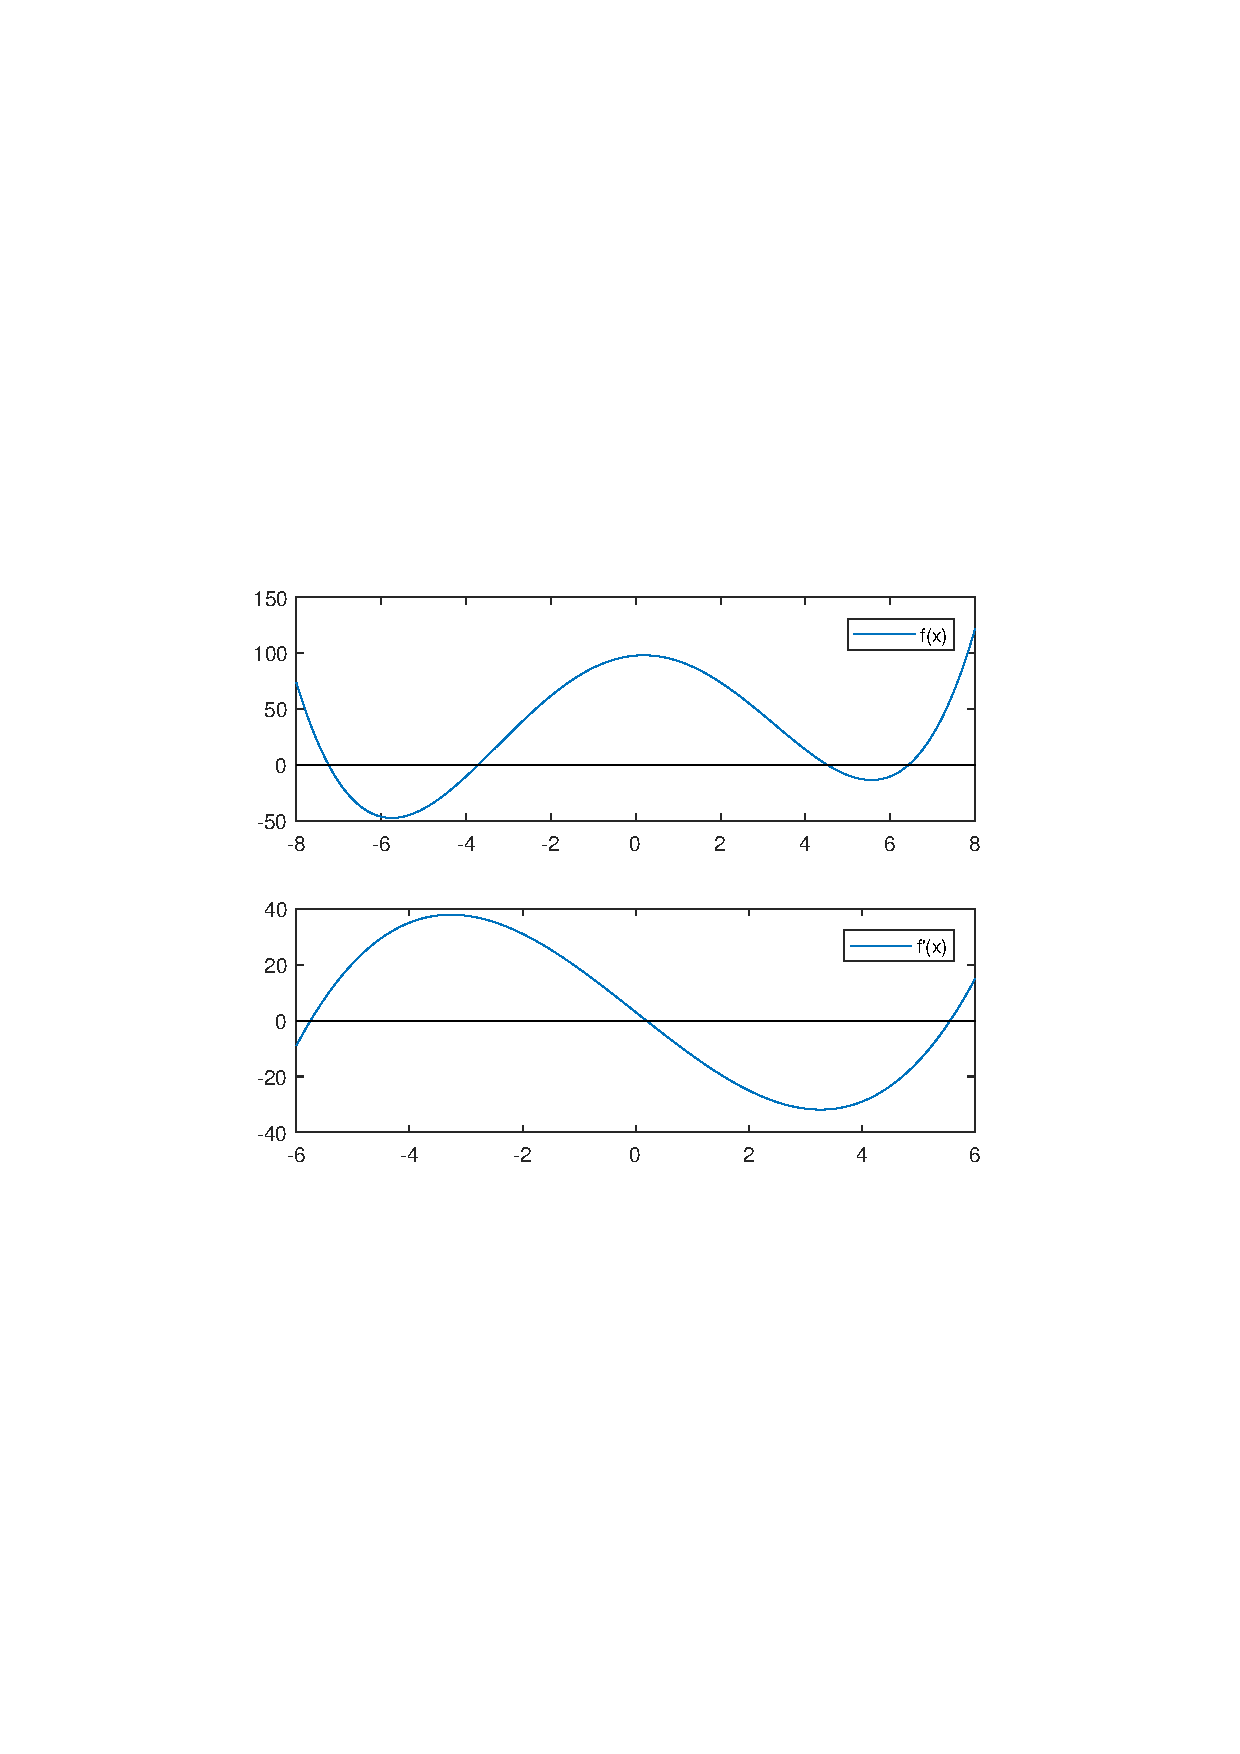
\includegraphics[width=11cm]{1.pdf}
\end{figure}

求解$f'(x)=0$得$x_1=-5.74837,x_2=0.187707,x_3=5.56066$,由于$x\geq 0$,故极小值在$x^{\star}=5.56066$处取到,此时无积极约束,$\mathcal{A}^{\star}=\emptyset$.

去掉约束条件$x \geq 0$后,
有两个局部极小点$x_1=-5.74837,x_3=5.56066$,其中全局极小点在$x_1$处取到.

\textbf{发现的结论:}去掉非积极约束对局部最优值没有影响,但可能会影响到全局最优解.

\item[7.3]
\[\mathcal{L}(\bm{x},\lambda)=(x_1-\dfrac{1}{9})^2+(x_2-2)^2+\lambda_1({x_1}^2-x_2)+\lambda_2(x_1+x_2-6)-\lambda_3x_1-\lambda_4x_2\]

\[\nabla_{\bm{x}}\mathcal{L}(\bm{x},\lambda)=\begin{bmatrix}
2(x_1-\dfrac{9}{4})+2\lambda_1x_1+\lambda_2-\lambda_3\\
2(x_2-2)-\lambda_1+\lambda_2-\lambda_4
\end{bmatrix}\]

\begin{enumerate}
\item

\textbf{KKT条件:}
\begin{align}
2(x_1-\dfrac{9}{4})+2\lambda_1x_1+\lambda_2-\lambda_3&=0\nonumber\\
2(x_2-2)-\lambda_1+\lambda_2-\lambda_4&=0\nonumber\\
{x_1}^2-x_2&\leq 0\nonumber\\
x_1+x_2-6&\leq 0\nonumber\\
		x_1&\geq 0\nonumber\\
	x_2&\geq 0\nonumber\\
\lambda_1({x_1}^2-x_2)&=0\nonumber\\
\lambda_2(x_1+x_2-6)&=0\nonumber\\
\lambda_3x_1&=0\nonumber\\
\lambda_4x_2&=0\nonumber\\
\lambda_i\geq0 ,\quad i&=1,2,3,4.\nonumber\\
\end{align}

代入$\bm{x}^{\star}=(\dfrac{3}{2},\dfrac{9}{4})^T$,其满足约束条件且解得:

\[\lambda_1=\dfrac{1}{2},\quad \lambda_2=\lambda_3=\lambda_4=0\]

\item
在$\bm{x}^{\star}$处的$\mathcal{A}^{\star}=\{1\}$。即在该点处$c_1(x)=0$与目标函数的等高线相切
\item
目标函数是凸函数,可行域是凸集,所以是凸规划,故局部极小点就是全局最优解.
\end{enumerate}
\item[7.4]
\begin{enumerate}
\item
设费用函数是$f(x)$,表述成优化问题为;
\begin{alignat}{2}
min \quad & f(\bm{x})=8{x_1}{x_2} +8{x_2}{x_3} +18{x_1}{x_3} \nonumber\\
\mbox{s.t.}\quad
&{x_1}{x_2}{x_3} - 1500= 0 \nonumber\\
&{x_1} - 2{x_2} = 0 \nonumber \\
&{x_1} \geq {x_2}  \nonumber 
\end{alignat}

\[\mathcal{L}(\bm{x},\lambda)=8{x_1}{x_2} + 8{x_2}{x_3} + 18{x_1}{x_3} + {\lambda _1}\left( {{x_1}{x_2}{x_3} - 1500} \right) + {\lambda _2}\left( {{x_1} - 2{x_2}}\right)+{\lambda _3}\left( {{x_2} - {x_1}} \right)\]

\[\nabla_{\bm{x}}\mathcal{L}(\bm{x},\lambda)=\begin{bmatrix}
8{x_2} + 18{x_3} + {\lambda _1}{x_2}{x_3} + {\lambda _2}- {\lambda _3}\\
8{x_1} +8{x_3} + {\lambda _1}{x_1}{x_3} - 2{\lambda _2}+{\lambda _3}\\
8{x_2} + 18{x_1} + {\lambda _1}{x_1}{x_2}\\
\end{bmatrix}\]


\textbf{KKT条件:}
\begin{align}
8{x_2} + 18{x_3} + {\lambda _1}{x_2}{x_3} + {\lambda _2}- {\lambda _3}&=0\nonumber\\
8{x_1} +8{x_3} + {\lambda _1}{x_1}{x_3} - 2{\lambda _2}+{\lambda _3}&=0\nonumber\\
8{x_2} + 18{x_1} + {\lambda _1}{x_1}{x_2}&=0\nonumber\\
{x_1}{x_2}{x_3} - 1500&=0\nonumber\\
{x_1} - 2{x_2}&=0\nonumber\\
{\lambda _3}( {{x_2} - {x_1}})&=0\nonumber\\
{\lambda _3}&\geq 0\nonumber\\
\end{align}

由等式约束${x_1}{x_2}{x_3} - 1500=0,\quad {x_1} - 2{x_2}=0$代入原问题确定:
\[\bm{x}_2^{\star}=10\sqrt[3]{\dfrac{33}{32}},\qquad \bm{\lambda}^{\star}=(\lambda_1^{\star},\lambda_2^{\star},\lambda_3^{\star})^T=(-\dfrac{22}{x_2^{\star}},-8x_2^{\star}+-\dfrac{3000}{{x_2^{\star}}^2},0)^T\]

\item
在原问题中消去$x_1,x_2$得;
\begin{alignat}{2}
min \quad & f(\bm{x})=16{x_2}^2+\dfrac{33000}{x_2} \nonumber\\
\mbox{s.t.}\quad
&x_2\geq 0 \nonumber\\
\end{alignat}

最优解为$x_2^{\star}=10\sqrt[3]{\dfrac{33}{32}}=10.1031$,
$\quad f(10)=4900,\quad f(11)=4936$,故最优整数解为$x_2=10,\quad \bm{x}^{\star}=(20,10,7.5)$

\item
解得:
\[\bm{x}(\varepsilon )=\left[
2x_2,
\sqrt[3]{{\frac{{33000 + 22\varepsilon }}{{32}}}},
\frac{{1500 + \varepsilon }}{{2{x_2}^2}}\right]^T\]
\[h(\varepsilon ) = 16{({x_{2}}(\varepsilon ))^2} + \frac{{33000 + 22\varepsilon }}{{{x_{ 2}}(\varepsilon )}}-f(\bm{x}^{\star})\]
\[h'(0) = \dfrac{{22}}{{{x_2}^{\star}}}=-\lambda_1^{\star}\]

$h(-150)=-332.3,\quad {\lambda_1}^{\star}\varepsilon =-326.6$,两者比较接近。
\end{enumerate}
\end{enumerate}
\end{document}